\documentclass[a4paper, 12pt, margins=3cm]{homework}
\usepackage{tikz}

\usepackage{graphicx}
\usepackage{dsfont}
\usepackage{microtype}
\usepackage{mathrsfs}
\usepackage[ngerman]{babel}
\usepackage{csquotes}
\usepackage[T1]{fontenc}
\usepackage{lmodern}
\usepackage{wasysym}

\name{Tobias Eidelpes}
\course{Formale Modellierung}
\term{2015WS}
\hwnum{2}
\hwtype{Übungsblatt}
\problemtitle{Aufgabe}
\solutiontitle{Lösung}

\begin{document}

\begin{problem}
  Sei $\mathcal{A}$ der folgende Mealy-Automat:
  \begin{center}
    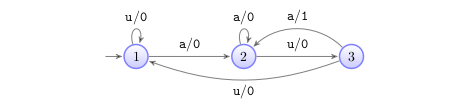
\includegraphics[scale=0.8]{automat.png}
  \end{center}
  \begin{parts}
    \part 
    \label{1.a}
    Geben Sie die Ausgabe zur Eingabe \texttt{uuaauauaauaaa} an.
    \part 
    \label{1.b}
    Beschreiben Sie $\mathcal{A}$ als 6-Tupel; legen Sie die Übergangsfunktion
    $\delta$ sowie die Ausgabefunktion $\gamma$ durch eine Tabelle fest.
    \part 
    \label{1.c}
    Berechnen Sie schrittweise $\delta \text{*}(1,\texttt{uauau})$ und $\gamma \text{*}(1,\texttt{uauau})$.
    \part 
    \label{1.d}
    Beschreiben Sie die Übersetzungsfunktion $[\mathcal{A}]$
  \end{parts}
\end{problem}
\begin{solution}
  \ref{1.a}
  Ausgabe zu \texttt{uuaauauaauaaa}: 0000010100100 \\

  \ref{1.b}
  \[ \mathcal{A} = \langle \{1,2,3\}, \{a,u\}, \{0,1\}, \delta, \gamma, 1 \rangle \]

  \begin{minipage}{0.5\textwidth}
    \begin{center}
      \begin{tabular}{c|cc}
        $\delta$ & a & u \\ \hline
        1        & 2 & 1 \\
        2        & 2 & 3 \\
        3        & 2 & 1
      \end{tabular}
    \end{center}
  \end{minipage}
  \begin{minipage}{0.5\textwidth}
    \begin{center}
      \begin{tabular}{c|cc}
        $\gamma$ & a & u \\ \hline
        1        & 0 & 0 \\
        2        & 0 & 0 \\
        3        & 1 & 0
      \end{tabular}
    \end{center}
  \end{minipage}

  \ref{1.c} \\

  \begin{minipage}{0.5\textwidth}
    \begin{center}
      \begin{align*}
        \delta\text{*}(1, uauau) &= \delta\text{*}(\delta(1,u), auau) \\
        &= \delta\text{*}(1, auau) \\
        &= \delta\text{*}(\delta(1,a), uau) \\
        &= \delta\text{*}(2, uau) \\
        &= \delta\text{*}(\delta(2,u), au) \\
        &= \delta\text{*}(3, au) \\
        &= \delta\text{*}(\delta(3,a), u) \\
        &= \delta\text{*}(2, u) \\
        &= \delta\text{*}(\delta(2,u), \varepsilon) \\
        &= \delta\text{*}(3, \varepsilon) \\
        &= 3
      \end{align*}
    \end{center}
  \end{minipage}
  \begin{minipage}{0.5\textwidth}
    \begin{center}
      \begin{align*}
        \gamma\text{*}(1, uauau) &= \gamma\text{*}(\gamma(1, u), auau) \\
        &= \gamma\text{*}(\gamma(1, a), uau) \\
        &= \gamma\text{*}(\gamma(2, u), au) \\
        &= \gamma\text{*}(\gamma(3, a), u) \\
        &= \gamma\text{*}(\gamma(2, u), \varepsilon) \\
        &= \gamma\text{*}(3, \varepsilon) \\
        &= \varepsilon
      \end{align*}
    \end{center}
  \end{minipage}
\end{solution}

\begin{problem}
  Finden Sie einen Moore-Automaten, der äquivalent zum Mealy-Automaten aus Aufgabe
  1 ist. Geben Sie ein Verfahren an, mit dem sich zu jedem Mealy-Automaten ein
  äquivalenter Moore-Automat konstruieren lässt.
\end{problem}
\begin{solution}
  Zuerst wird die Ausgabe in die jeweiligen Knoten geschrieben. Dann werden die 
  Zustände vervielfacht, damit jedem Zustand nur ein Ausgabewert zugeordnet ist.
  Danach eingehende Kanten zu den entsprechenden Zuständen umhängen und zu guter
  Letzt ausgehende Kanten vervielfachen und an die vervielfachten Zustände hängen.
  \begin{center}
    \begin{tikzpicture}[scale=0.2]
      \tikzstyle{every node}+=[inner sep=0pt]
      \draw [black] (22.5,-14.4) circle (3);
      \draw (22.5,-14.4) node {$\frac{1}{0}$};
      \draw [black] (41.5,-14.4) circle (3);
      \draw (41.5,-14.4) node {$\frac{2}{0}$};
      \draw [black] (60.3,-14.4) circle (3);
      \draw (60.3,-14.4) node {$\frac{3}{0}$};
      \draw [black] (60.3,-31.4) circle (3);
      \draw (60.3,-31.4) node {$\frac{2}{1}$};
      \draw [black] (25.5,-14.4) -- (38.5,-14.4);
      \fill [black] (38.5,-14.4) -- (37.7,-13.9) -- (37.7,-14.9);
      \draw (32,-13.9) node [above] {$a$};
      \draw [black] (40.177,-11.72) arc (234:-54:2.25);
      \draw (41.5,-7.15) node [above] {$a$};
      \fill [black] (42.82,-11.72) -- (43.7,-11.37) -- (42.89,-10.78);
      \draw [black] (44.5,-14.4) -- (57.3,-14.4);
      \fill [black] (57.3,-14.4) -- (56.5,-13.9) -- (56.5,-14.9);
      \draw (50.9,-14.9) node [below] {$u$};
      \draw [black] (58.06,-16.393) arc (-51.54099:-128.45901:26.787);
      \fill [black] (24.74,-16.39) -- (25.06,-17.28) -- (25.68,-16.5);
      \draw (41.4,-22.7) node [below] {$u$};
      \draw [black] (60.3,-17.4) -- (60.3,-28.4);
      \fill [black] (60.3,-28.4) -- (60.8,-27.6) -- (59.8,-27.6);
      \draw (59.8,-22.9) node [left] {$a$};
      \draw [black] (10.4,-14.4) -- (19.5,-14.4);
      \fill [black] (19.5,-14.4) -- (18.7,-13.9) -- (18.7,-14.9);
      \draw [black] (21.177,-11.72) arc (234:-54:2.25);
      \draw (22.5,-7.15) node [above] {$u$};
      \fill [black] (23.82,-11.72) -- (24.7,-11.37) -- (23.89,-10.78);
    \end{tikzpicture}
  \end{center}
\end{solution}
\end{document}